\section{CP}

The first technique used to approach the problem was modeling with CP (Constraint Programming) using Minizinc.

For clarification purposes, we report the structure of each input instance encoded in a \textit{.dzn} file, which is readable by MiniZinc:

$w = {width} \\
n = {number \; of \; circuits} \\
x\_dim = [{x_0}, \; {x_1}, \; ..., \; {x_n}] \\
y\_dim = [{y_0}, \; {y_1}, \; ..., \; {y_n}]$ 

\subsection{Variables}

First of all, all the parameters, decision variables and objective variables of the problem had to be defined. 

The \textbf{input and output parameters} were the ones previously described in the introduction, which were defined in the model using the MiniZinc syntax.

We want to model our variables to have the smallest possible domain in order to reduce the search space. Hence, we reduced the variable domain to make the model more efficient. This was done by defining a range for each variable of the array $x$: the bottom left corner of each rectangle $i$ cannot be placed farther along the x axis than the plate width minus its horizontal dimension, otherwise it would fall outside the plate. A similar reasoning can be defined for the domain of the variables $y_i$: the bottom left corner of each rectangle $i$ cannot be placed higher on the y axis than the height of the plate minus its vertical dimension.

\begin{equation*}
    \forall i \in \{1..n\} \quad x_i \leq width - x\_dim_i
\end{equation*}

\begin{equation*}
    \forall i \in \{1..n\} \quad y_i \leq height - y\_dim_i
\end{equation*}

Moreover, with the same purpose of reducing variables domain, upper and lower bounds were defined for the plate's height:
\begin{itemize}
    \item lower bound: the plate's height cannot be smaller than the height of the tallest rectangle
    \[ lowb = max(y\_dim_i) \quad \forall i \in \{1..n\}\]
    \item upper bound: the plate's height must be below the sum of all the rectangles' heights
    \[upb = sum(y\_dim_i) \quad \forall i \in \{1..n\} \]
\end{itemize}

\hfill

\subsection{Objective function}

The \textbf {objective function} is to minimize the objective variable \textit{height}, which is the height of the plate. 

It ranges from the lower bound \textit{lowb} to the upper bound \textit{upb} which were previously described and it is defined as:

\begin{equation*}
    height = max(y_i + y\_dim_i \; | \; i \in \{1..n\} )
\end{equation*}

\subsection{Constraints}

One of the most important parts of the problem is related to the definition of different constraints and their propagation in order to remove inconsistent values from variables domain.

The use of \textbf{global constraints} is useful for the solution of this problem, since it allows to obtain more efficient solutions thanks to propagation algorithms. Two different global constraints were used: \textbf {cumulative} and \textbf {diffn}. 

The \textit{cumulative} constraint was taken from the modeling of scheduling problems: it is usually used when we want to constrain the usage of shared resources by different tasks. In general, it requires that a set of tasks given by start times \textbf{s}, durations \textbf{d} and resource requirements \textbf{r} never require more than a global resource bound \textbf{b} at any one time. 

Our problem can be seen as one of this kind. More specifically, for the x axis, the plate’s height represents the resource
bound and each circuit is a task where its x coordinate represents the starting time, its width represents the duration, while the circuit's height represents the required
resource. The same reasoning can be applied symmetrically for the y axis.

\begin{verbatim}
cumulative(x, x_dim, y_dim, height)
cumulative(y, y_dim, x_dim, width)
\end{verbatim}

The \textit{diffn} constraint is a non-overlapping constraint which, given the vectors of circuits' bottom-left coordinates $x$ and $y$ and the vectors of their dimensions $x\_dim$ and $y\_dim$, it prevents the circuits from overlapping:

\begin{verbatim}
diffn(x, y, x_dim, y_dim)
\end{verbatim}


Furthermore, \textbf{symmetry braking constraints} were applied to reduce the number of solutions: the solver may in fact explore many symmetric variants of the same solution. The basic idea behind symmetry breaking is to impose an order.
In our case it was decided to place always the biggest circuit in the bottom left part of the plate. The rationale behind this choice is that, by taking up the most space on the plate, it is the most likely circuit to have an impact on the positioning of subsequent circuits.

To do this we need to define an order of the circuits, which is done by sorting them in descending order considering their area, given by the product between $x\_dim$ and $y\_dim$. We call \verb|ord_circ| the array of sorted circuits by their area. 

After that, we force the x and y coordinates of the bottom-left corner of the biggest circuit to be 0, meaning that it will be placed in the bottom-left part of the plate:

\begin{equation*}
    \verb|x[ord_circ[1]] = 0| \; \land \; \verb|y[ord_circ[1]] = 0|
\end{equation*}

\subsection{Rotation model}

If we decide to take into account the rotation of the circuits, we need to perform some model modifications. This is done by introducing a boolean array \verb|rotation| indexed by the number of circuits which specifies if each circuit is rotated or not.

In case of rotation each rectangle will have its width and height values swapped, therefore we need to update their actual values of widths and heights accordingly:

\begin{equation*}
\forall i \; \in \; \{1..n\} \quad \; x\_dim\_rot_i  = \begin{cases} y\_dim_i & \mbox{if } \mbox{rotation$_i$} \\ x\_dim_i & \mbox{otherwise}\end{cases}
\end{equation*}

\begin{equation*}
\forall i \; \in \; \{1..n\} \quad \; y\_dim\_rot_i  = \begin{cases} x\_dim_i & \mbox{if } \mbox{rotation$_i$} \\ y\_dim_i & \mbox{otherwise}\end{cases}
\end{equation*}

As a consequence, the objective variable \textit{height} and the constraints seen before are modified by simply replacing the original dimension variables with $x\_dim\_rot$ and $y\_dim\_rot$ to allow rotation. 

We also introduce a new constraint, which says that a circuit cannot be rotated if its height is greater than the plate's width:

\begin{equation*}
    \forall i \in \{1..n\} \quad y\_dim_i > width \implies rotation_i = false
\end{equation*}

Moreover, another symmetry braking constraint is added due to the fact that, in case of rectangles which are squares (meaning that they have the same dimensions), we avoid the rotation forcing width and height to be the original ones.

\begin{equation*}
     \forall i \in \{1..n\} \quad x\_dim_i = y\_dim_i \implies (x\_dim\_rot_i = x\_dim_i \land y\_dim\_rot_i = y\_dim_i)
\end{equation*}

The output file is also modified so that the string \textit{"rotated"} is printed next to the coordinates of the output circuits: this indicates that the related circuit has been rotated. 

As an example, a possible output for the instance 3 is the following:

$ 10 \quad 10 \\
6 \\
3 \quad 3 \quad 4 \quad 7 \\
3 \quad 4 \quad 0 \quad 7 \quad rotated \\
3 \quad 6 \quad 7 \quad 4 \\
3 \quad 7 \quad 0 \quad 4 \quad rotated \\
4 \quad 4 \quad 6 \quad 0 \\
4 \quad 6 \quad 0 \quad 0 \quad rotated $ 


\subsection{Hardware setup}

The experiments were performed on a machine with the following specifications:

\begin{itemize}
    \item Apple M1 Pro 8-core
    \item 16 GB of RAM 
    \item macOS 13.0
\end{itemize}

The project was developed using Python 3.10.6 and MiniZinc 2.6.4.

\subsection{Validation}

The model was implemented with MiniZinc and run using Gecode solver. Different combinations of search heuristics, for variables and domains, as well as restart strategies were employed to compare the model performances. In particular, as variables heuristics we considered:
\begin{itemize}
    \item \textit{input\_order}, that chooses the variable in order from the array
    \item \textit{first\_fail}, that chooses the variable with the smallest domain size
    \item \textit{dom\_w\_deg}, that chooses the variable with the smallest value of domain size divided by weighted degree, which is the number of times it has been in a constraint that caused failure earlier in the search
\end{itemize}

As domain heuristic, the choice was made on \textit{indomain\_min}, that assigns the variable with its smallest domain value.

Also, restarting the search is useful to introduce randomness and break deterministic behaviour in searching solutions. In the model, different restart strategies were chosen:
\begin{itemize}
    \item restart\_constant(100)
    \item restart\_linear(100)
    \item restart\_geometric(1.5, 100)
    \item restart\_luby(100)
\end{itemize}

\begin{figure}[!tbp]
  \centering
  \subfloat[Solution without rotation]{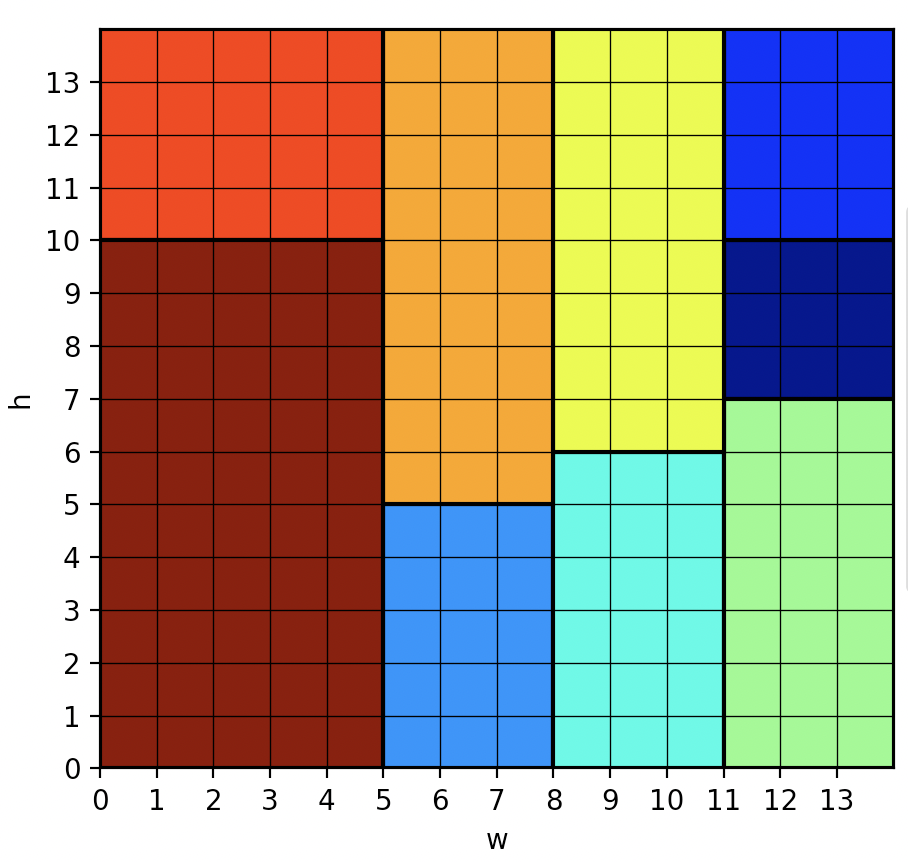
\includegraphics[width=0.4\textwidth]{Images/ins-7.png}\label{fig:f1}}
  \hfill
  \subfloat[Solution with rotation]{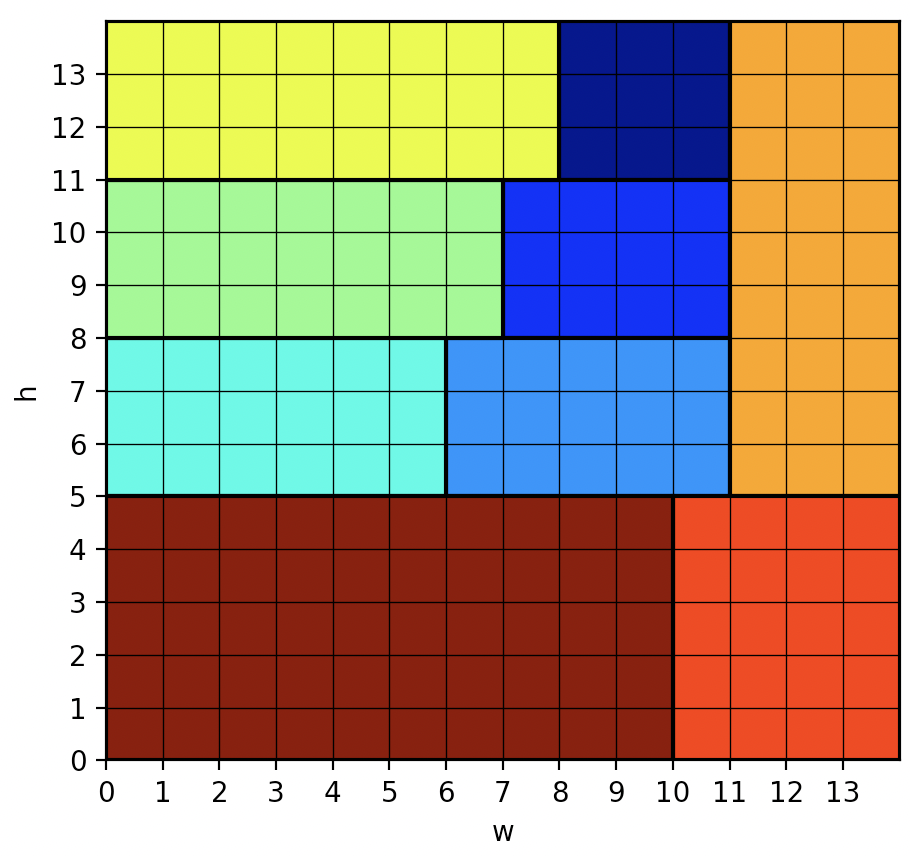
\includegraphics[width=0.4\textwidth]{Images/ins-7-rot.png}\label{fig:f2}}
  \hfill
  \subfloat[Legend of circuits]{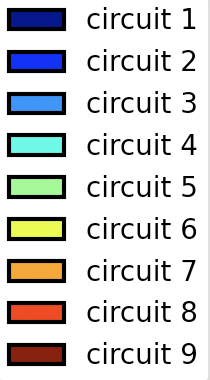
\includegraphics[width=0.1\textwidth]{Images/ins-7-legend.png}\label{fig:f3}}
  \caption{Example of a possible solution for the instance n. 7}
\end{figure}


The results compare the performances of the base model (no rotation) and of the rotation model, both tested with and without symmetry braking constraints.

During the experiments, a time limit of 300 seconds was imposed: if the solver was not able to find a solution within the time limit, the solving process was aborted.

After experimenting with different combinations, the search strategy configuration which produced the best trade-off between the number of solved instances and solving time was \textit{input\_order} and \textit{indomain\_min} combined with \textit{geometric restart}. The results are shown in Table 1.


\begin{center}
\begin{longtable}{|l|l|l|l|l|l|}
\caption{Solving times and height obtained by CP models (base and rotation) with and without symmetry braking constraints} \label{tab:long} \\

\hline \multicolumn{1}{|c|}{\textbf{Instance}} & \multicolumn{1}{c|}{\textbf{Base + SB}} & \multicolumn{1}{c|}{\textbf{Base w/o SB}} & \multicolumn{1}{c|}{\textbf{Rot + SB}} & \multicolumn{1}{c|}{\textbf{Rot w/o SB}} & \multicolumn{1}{c|}{\textbf{Height}} \\ \hline 
\endfirsthead

\multicolumn{6}{c}
{{\bfseries \tablename\ \thetable{} -- continued from previous page}} \\
\hline \multicolumn{1}{|c|}{\textbf{Instance}} & \multicolumn{1}{c|}{\textbf{Base w/ SB}} & \multicolumn{1}{c|}{\textbf{Base w/o SB}} & \multicolumn{1}{c|}{\textbf{Rot w/ SB}} & \multicolumn{1}{c|}{\textbf{Rot w/o SB}} & \multicolumn{1}{c|}{\textbf{Height}} \\ \hline 
\endhead

\hline \multicolumn{6}{|r|}{{Continued on next page}} \\ \hline
\endfoot

\hline \hline
\endlastfoot

1 & 0,194 & 0,287 & 0,268 & 0,217 & 8 \\
2 & 0,192 & 0,202 & 0,219 & 0,219 & 9 \\
3 & 0,196 & 0,205 & 0,206 & 0,217 & 10 \\
4 & 0,192 & 0,207 & 0,246 & 0,312 & 11 \\
5 & 0,212 & 0,208 & 1,354 & 0,255 & 12 \\
6 & 0,200 & 0,213 & 1,165 & 1,499 & 13 \\
7 & 0,228 & 0,206 & 3,688 & 46,06 & 14 \\
8 & 0,235 & 0,235 & 0,225 & 0,212 & 15 \\
9 & 0,198 & 0,207 & 19,26 & 87,64 & 16 \\
10 & 0,199 & 0,210 & - & - & 17 \\
11 & 0,203 & 0,206 & - & - & 18 \\
12 & 0,228 & 0,218 & 0,523 & 0,224 & 19 \\
13 & 0,202 & 0,204 & - & - & 20 \\
14 & 0,222 & 0,231 & - & - & 21 \\
15 & 0,193 & 0,250 & 0,266 & 0,227 & 22 \\
16 & 1,317 & - & - & - & 23 \\
17 & 6,366 & 6,158 & 0,236 & 0,215 & 24 \\
18 & 1,434 & 1,436 & 1,120  & - & 25 \\
19 & - & - & - & - & - \\
20 & 5,908 & 5,771 & - & - & 27 \\
21 & 0,227 & 0,211 & - & - & 28 \\
22 & - & - & - & - & - \\
23 & 0,266 & - & - & - & 30 \\
24 & 0,231 & 20,68 & 0,228 & 0,309 & 31 \\
25 & - & - & - & - & - \\
26 & 147,4 & - & 0,918 & - & 33 \\
27 & 0,233 & 60,50 & 0,221 & 0,286 & 34 \\
28 & 17,23 & - & - & - & 35 \\
29 & 0,246 & - & - & - & 36 \\
30 & - & - & - & - & - \\
31 & - & - & 271,7 & - & 38 \\
32 & - & - & - & - & - \\
33 & 0,231 & 0,309 & 0,242 & 0,218 & 40 \\
34 & - & - & - & - & - \\
35 & - & - & - & - & - \\
36 & 0,232 & 0,278 & - & - & 40 \\
37 & - & - & - & - & - \\
38 & - & - & - & - & - \\
39 & - & - & - & - & - \\
40 & - & - & - & - & - \\
\end{longtable}
\end{center}


\newpage